
%(BEGIN_QUESTION)
% Copyright 2015, Tony R. Kuphaldt, released under the Creative Commons Attribution License (v 1.0)
% This means you may do almost anything with this work of mine, so long as you give me proper credit

This protective relay circuit has a problem.  During the last fault, it successfully tripped the circuit breaker, but the relay never registered the change in breaker status (from closed to tripped) -- instead it continued to show the breaker as remaining in the {\it closed} state.  The indicator lamp functions just fine.

$$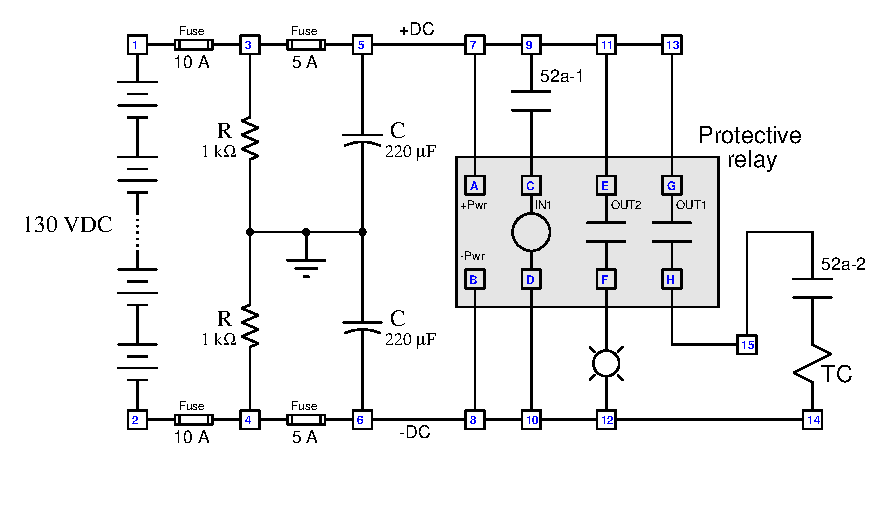
\includegraphics[width=15.5cm]{i03100x01.eps}$$

Identify the likelihood of each specified fault for this circuit.  Consider each fault one at a time (i.e. no coincidental faults), determining whether or not each fault could independently account for {\it all} measurements and symptoms in this circuit.

% No blank lines allowed between lines of an \halign structure!
% I use comments (%) instead, so that TeX doesn't choke.

$$\vbox{\offinterlineskip
\halign{\strut
\vrule \quad\hfil # \ \hfil & 
\vrule \quad\hfil # \ \hfil & 
\vrule \quad\hfil # \ \hfil \vrule \cr
\noalign{\hrule}
%
% First row
{\bf Fault} & {\bf Possible} & {\bf Impossible} \cr
%
\noalign{\hrule}
%
% Another row
Battery bank voltage low &  & \cr
%
\noalign{\hrule}
%
% Another row
52a-1 contact failed open &  & \cr
%
\noalign{\hrule}
%
% Another row
52a-1 contact failed shorted &  & \cr
%
\noalign{\hrule}
%
% Another row
Failed relay input IN1 &  & \cr
%
\noalign{\hrule}
%
% Another row
Trip coil failed open &  & \cr
%
\noalign{\hrule}
%
% Another row
Trip coil failed shorted &  & \cr
%
\noalign{\hrule}
%
% Another row
Wire between terminals 5 and 7 failed open &  &  \cr
%
\noalign{\hrule}
%
% Another row
Wire between terminals 9 and 11 failed open &  &  \cr
%
\noalign{\hrule}
%
% Another row
Wire between terminals 10 and D failed open &  &  \cr
%
\noalign{\hrule}
} % End of \halign 
}$$ % End of \vbox

Finally, identify the {\it next} diagnostic test or measurement you would make on this system.  Explain how the result(s) of this next test or measurement help further identify the location and/or nature of the fault.

\underbar{file i03100}
%(END_QUESTION)





%(BEGIN_ANSWER)

 
%(END_ANSWER)





%(BEGIN_NOTES)

% No blank lines allowed between lines of an \halign structure!
% I use comments (%) instead, so that TeX doesn't choke.

$$\vbox{\offinterlineskip
\halign{\strut
\vrule \quad\hfil # \ \hfil & 
\vrule \quad\hfil # \ \hfil & 
\vrule \quad\hfil # \ \hfil \vrule \cr
\noalign{\hrule}
%
% First row
{\bf Fault} & {\bf Possible} & {\bf Impossible} \cr
%
\noalign{\hrule}
%
% Another row
Battery bank voltage low &  & $\surd$ \cr
%
\noalign{\hrule}
%
% Another row
52a-1 contact failed open &  & $\surd$ \cr
%
\noalign{\hrule}
%
% Another row
52a-1 contact failed shorted & $\surd$ & \cr
%
\noalign{\hrule}
%
% Another row
Failed relay input IN1 & $\surd$ &  \cr
%
\noalign{\hrule}
%
% Another row
Trip coil failed open &  & $\surd$ \cr
%
\noalign{\hrule}
%
% Another row
Trip coil failed shorted &  & $\surd$ \cr
%
\noalign{\hrule}
%
% Another row
Wire between terminals 5 and 7 failed open &  & $\surd$ \cr
%
\noalign{\hrule}
%
% Another row
Wire between terminals 9 and 11 failed open &  & $\surd$ \cr
%
\noalign{\hrule}
%
% Another row
Wire between terminals 10 and D failed open &  & $\surd$ \cr
%
\noalign{\hrule}
} % End of \halign 
}$$ % End of \vbox

A good ``next test'' would be to measure voltage at the relay's IN1 input terminals: between terminals C and D.  The presence of voltage (with the breaker tripped) indicates a shorted 52a-1 contact.  The absence of voltage indicates a failed relay input.

%INDEX% Protective relay: troubleshooting

%(END_NOTES)


